% Options for packages loaded elsewhere
\PassOptionsToPackage{unicode}{hyperref}
\PassOptionsToPackage{hyphens}{url}
%
\documentclass[
]{article}
\usepackage{amsmath,amssymb}
\usepackage{iftex}
\ifPDFTeX
  \usepackage[T1]{fontenc}
  \usepackage[utf8]{inputenc}
  \usepackage{textcomp} % provide euro and other symbols
\else % if luatex or xetex
  \usepackage{unicode-math} % this also loads fontspec
  \defaultfontfeatures{Scale=MatchLowercase}
  \defaultfontfeatures[\rmfamily]{Ligatures=TeX,Scale=1}
\fi
\usepackage{lmodern}
\ifPDFTeX\else
  % xetex/luatex font selection
\fi
% Use upquote if available, for straight quotes in verbatim environments
\IfFileExists{upquote.sty}{\usepackage{upquote}}{}
\IfFileExists{microtype.sty}{% use microtype if available
  \usepackage[]{microtype}
  \UseMicrotypeSet[protrusion]{basicmath} % disable protrusion for tt fonts
}{}
\makeatletter
\@ifundefined{KOMAClassName}{% if non-KOMA class
  \IfFileExists{parskip.sty}{%
    \usepackage{parskip}
  }{% else
    \setlength{\parindent}{0pt}
    \setlength{\parskip}{6pt plus 2pt minus 1pt}}
}{% if KOMA class
  \KOMAoptions{parskip=half}}
\makeatother
\usepackage{xcolor}
\usepackage[top=100pt,bottom=100pt,left=68pt,right=66pt]{geometry}
\usepackage{color}
\usepackage{fancyvrb}
\newcommand{\VerbBar}{|}
\newcommand{\VERB}{\Verb[commandchars=\\\{\}]}
\DefineVerbatimEnvironment{Highlighting}{Verbatim}{commandchars=\\\{\}}
% Add ',fontsize=\small' for more characters per line
\usepackage{framed}
\definecolor{shadecolor}{RGB}{248,248,248}
\newenvironment{Shaded}{\begin{snugshade}}{\end{snugshade}}
\newcommand{\AlertTok}[1]{\textcolor[rgb]{0.94,0.16,0.16}{#1}}
\newcommand{\AnnotationTok}[1]{\textcolor[rgb]{0.56,0.35,0.01}{\textbf{\textit{#1}}}}
\newcommand{\AttributeTok}[1]{\textcolor[rgb]{0.13,0.29,0.53}{#1}}
\newcommand{\BaseNTok}[1]{\textcolor[rgb]{0.00,0.00,0.81}{#1}}
\newcommand{\BuiltInTok}[1]{#1}
\newcommand{\CharTok}[1]{\textcolor[rgb]{0.31,0.60,0.02}{#1}}
\newcommand{\CommentTok}[1]{\textcolor[rgb]{0.56,0.35,0.01}{\textit{#1}}}
\newcommand{\CommentVarTok}[1]{\textcolor[rgb]{0.56,0.35,0.01}{\textbf{\textit{#1}}}}
\newcommand{\ConstantTok}[1]{\textcolor[rgb]{0.56,0.35,0.01}{#1}}
\newcommand{\ControlFlowTok}[1]{\textcolor[rgb]{0.13,0.29,0.53}{\textbf{#1}}}
\newcommand{\DataTypeTok}[1]{\textcolor[rgb]{0.13,0.29,0.53}{#1}}
\newcommand{\DecValTok}[1]{\textcolor[rgb]{0.00,0.00,0.81}{#1}}
\newcommand{\DocumentationTok}[1]{\textcolor[rgb]{0.56,0.35,0.01}{\textbf{\textit{#1}}}}
\newcommand{\ErrorTok}[1]{\textcolor[rgb]{0.64,0.00,0.00}{\textbf{#1}}}
\newcommand{\ExtensionTok}[1]{#1}
\newcommand{\FloatTok}[1]{\textcolor[rgb]{0.00,0.00,0.81}{#1}}
\newcommand{\FunctionTok}[1]{\textcolor[rgb]{0.13,0.29,0.53}{\textbf{#1}}}
\newcommand{\ImportTok}[1]{#1}
\newcommand{\InformationTok}[1]{\textcolor[rgb]{0.56,0.35,0.01}{\textbf{\textit{#1}}}}
\newcommand{\KeywordTok}[1]{\textcolor[rgb]{0.13,0.29,0.53}{\textbf{#1}}}
\newcommand{\NormalTok}[1]{#1}
\newcommand{\OperatorTok}[1]{\textcolor[rgb]{0.81,0.36,0.00}{\textbf{#1}}}
\newcommand{\OtherTok}[1]{\textcolor[rgb]{0.56,0.35,0.01}{#1}}
\newcommand{\PreprocessorTok}[1]{\textcolor[rgb]{0.56,0.35,0.01}{\textit{#1}}}
\newcommand{\RegionMarkerTok}[1]{#1}
\newcommand{\SpecialCharTok}[1]{\textcolor[rgb]{0.81,0.36,0.00}{\textbf{#1}}}
\newcommand{\SpecialStringTok}[1]{\textcolor[rgb]{0.31,0.60,0.02}{#1}}
\newcommand{\StringTok}[1]{\textcolor[rgb]{0.31,0.60,0.02}{#1}}
\newcommand{\VariableTok}[1]{\textcolor[rgb]{0.00,0.00,0.00}{#1}}
\newcommand{\VerbatimStringTok}[1]{\textcolor[rgb]{0.31,0.60,0.02}{#1}}
\newcommand{\WarningTok}[1]{\textcolor[rgb]{0.56,0.35,0.01}{\textbf{\textit{#1}}}}
\usepackage{graphicx}
\makeatletter
\def\maxwidth{\ifdim\Gin@nat@width>\linewidth\linewidth\else\Gin@nat@width\fi}
\def\maxheight{\ifdim\Gin@nat@height>\textheight\textheight\else\Gin@nat@height\fi}
\makeatother
% Scale images if necessary, so that they will not overflow the page
% margins by default, and it is still possible to overwrite the defaults
% using explicit options in \includegraphics[width, height, ...]{}
\setkeys{Gin}{width=\maxwidth,height=\maxheight,keepaspectratio}
% Set default figure placement to htbp
\makeatletter
\def\fps@figure{htbp}
\makeatother
\setlength{\emergencystretch}{3em} % prevent overfull lines
\providecommand{\tightlist}{%
  \setlength{\itemsep}{0pt}\setlength{\parskip}{0pt}}
\setcounter{secnumdepth}{5}
\usepackage{float}
\usepackage{longtable}
\usepackage{caption}
\usepackage{fancyhdr}
\usepackage{titling}
\renewcommand{\headrulewidth}{0pt}
\renewcommand{\and}{\\}
\pretitle{\centering\vspace{0cm}{732A51 Bioinformatics \par}\vspace{5cm}\Huge\textbf}
\posttitle{\vspace{1cm}\large\textbf{}\par}
\preauthor{\centering\vspace{4cm}\normalsize}
\postauthor{\par\vspace{2cm}}
\predate{\centering{\normalsize STIMA \\ Department of Computer and Information Science \\ Linköpings universitet \par}}
\postdate{\par\vspace{0cm}}
\raggedbottom
\ifLuaTeX
  \usepackage{selnolig}  % disable illegal ligatures
\fi
\usepackage{bookmark}
\IfFileExists{xurl.sty}{\usepackage{xurl}}{} % add URL line breaks if available
\urlstyle{same}
\hypersetup{
  pdftitle={LAB 5 Bioinformatics},
  pdfauthor={Hugo Morvan; William Wiik},
  hidelinks,
  pdfcreator={LaTeX via pandoc}}

\title{LAB 5 Bioinformatics}
\author{Hugo Morvan \and William Wiik}
\date{2024-12-13}

\begin{document}
\maketitle

\fancyhf{}
\fancyfoot[C]{\thepage}
\pagestyle{fancy}

\pagenumbering{gobble}

\clearpage

\setcounter{tocdepth}{3}
\tableofcontents

\clearpage

\pagenumbering{arabic}
\setcounter{page}{1}

\section{Question 1}\label{question-1}

Go to the webpage \url{http://snap.stanford.edu/biodata/} and choose one
of the provided datasets. Download it and reproduce the statistics
concerning the graph. If you obtain different values, then discuss this
in your report. Visualize the graph. The next step is to try to identify
some clusters (communities in the graph). You can follow the tutorial at
\url{https://psych-networks.com/r-tutorial-identify-communities-items-networks/}
to achieve this. Once you have found some clusters, identify the
elements in it and try to find information on this cluster. Is it
related to some known biological phenomena? If you do not find anything,
then document your search attempts. If it will not be possible to do
this question on the whole downloaded graph, then you may take some
sub-graph of it.

\begin{Shaded}
\begin{Highlighting}[]
\FunctionTok{library}\NormalTok{(qgraph)}
\FunctionTok{library}\NormalTok{(igraph)}
\FunctionTok{library}\NormalTok{(ape)}


\NormalTok{con }\OtherTok{\textless{}{-}} \FunctionTok{gzfile}\NormalTok{(}\StringTok{"X:/Desktop/Bioinformatics/Lab5/ChG{-}Miner\_miner{-}chem{-}gene.tsv.gz"}\NormalTok{, }\StringTok{"rt"}\NormalTok{)}
\NormalTok{data }\OtherTok{\textless{}{-}} \FunctionTok{read.table}\NormalTok{(con, }\AttributeTok{sep =} \StringTok{"}\SpecialCharTok{\textbackslash{}t}\StringTok{"}\NormalTok{, }\AttributeTok{header =} \ConstantTok{FALSE}\NormalTok{)}
\FunctionTok{close}\NormalTok{(con)}
\FunctionTok{colnames}\NormalTok{(data) }\OtherTok{\textless{}{-}} \FunctionTok{c}\NormalTok{(}\StringTok{"Drug"}\NormalTok{,}\StringTok{"Gene"}\NormalTok{)}

\NormalTok{g }\OtherTok{\textless{}{-}} \FunctionTok{graph\_from\_data\_frame}\NormalTok{(data, }\AttributeTok{directed =} \ConstantTok{TRUE}\NormalTok{)}
\NormalTok{g}
\end{Highlighting}
\end{Shaded}

\begin{verbatim}
## IGRAPH 43fec92 DN-- 7341 15138 -- 
## + attr: name (v/c)
## + edges from 43fec92 (vertex names):
##  [1] DB00357->P05108 DB02721->P00325 DB00773->P23219 DB07138->Q16539
##  [5] DB08136->P24941 DB01242->P23975 DB01238->P08173 DB00186->P48169
##  [9] DB00338->P10635 DB01151->P08913 DB01244->P05023 DB01745->P07477
## [13] DB01996->P08254 DB04800->P18031 DB08352->Q16539 DB00133->P21549
## [17] DB00163->P21266 DB00197->P10632 DB06777->P08684 DB01151->P10635
## [21] DB00356->P08684 DB01589->P34903 DB01272->P20645 DB08846->Q14534
## [25] DB01151->P33261 DB01076->P04035 DB00605->Q03181 DB08515->P49721
## [29] DB02401->P07195 DB01057->P06276 DB03286->P11217 DB08814->Q9Y233
## + ... omitted several edges
\end{verbatim}

\begin{Shaded}
\begin{Highlighting}[]
\CommentTok{\# Number of nodes and edges}
\FunctionTok{cat}\NormalTok{(}\StringTok{"Number of nodes:"}\NormalTok{, }\FunctionTok{vcount}\NormalTok{(g), }\StringTok{"}\SpecialCharTok{\textbackslash{}n}\StringTok{"}\NormalTok{)}
\end{Highlighting}
\end{Shaded}

\begin{verbatim}
## Number of nodes: 7341
\end{verbatim}

\begin{Shaded}
\begin{Highlighting}[]
\FunctionTok{cat}\NormalTok{(}\StringTok{"Number of edges:"}\NormalTok{, }\FunctionTok{ecount}\NormalTok{(g), }\StringTok{"}\SpecialCharTok{\textbackslash{}n}\StringTok{"}\NormalTok{)}
\end{Highlighting}
\end{Shaded}

\begin{verbatim}
## Number of edges: 15138
\end{verbatim}

\begin{Shaded}
\begin{Highlighting}[]
\FunctionTok{plot}\NormalTok{(g, }\AttributeTok{vertex.size=}\DecValTok{5}\NormalTok{,}\AttributeTok{vertex.label=}\ConstantTok{NA}\NormalTok{, }\AttributeTok{edge.width=}\FloatTok{0.01}\NormalTok{,}\AttributeTok{vertex.color=}\StringTok{"coral"}\NormalTok{, }\AttributeTok{main=}\StringTok{"ChG{-}Miner\_miner{-}chem{-}gene Graph"}\NormalTok{)}
\end{Highlighting}
\end{Shaded}

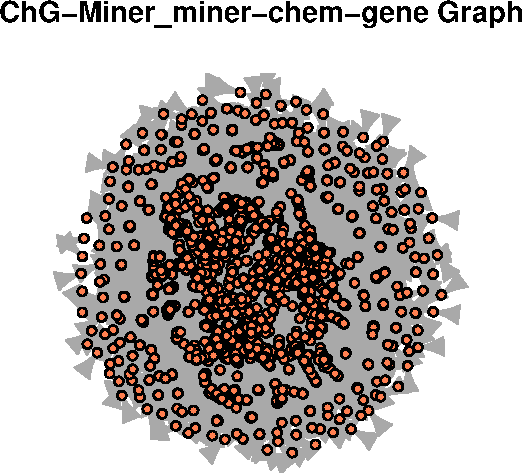
\includegraphics{lab5bio_files/figure-latex/unnamed-chunk-3-1.pdf}

\begin{Shaded}
\begin{Highlighting}[]
\CommentTok{\# Function to create and plot a bipartite network from an edge matrix}
\NormalTok{plot\_bipartite\_network }\OtherTok{\textless{}{-}} \ControlFlowTok{function}\NormalTok{(edge\_matrix, }\AttributeTok{title =} \StringTok{"Bipartite Network"}\NormalTok{,}\AttributeTok{plot\_graph =} \ConstantTok{TRUE}\NormalTok{, }\AttributeTok{top\_n =} \DecValTok{9}\NormalTok{) \{}
  \CommentTok{\# Create unique node names}
\NormalTok{  drugs }\OtherTok{\textless{}{-}} \FunctionTok{unique}\NormalTok{(edge\_matrix[,}\DecValTok{1}\NormalTok{])}
\NormalTok{  genes }\OtherTok{\textless{}{-}} \FunctionTok{unique}\NormalTok{(edge\_matrix[,}\DecValTok{2}\NormalTok{])}
  
  \CommentTok{\# Create the graph}
\NormalTok{  g }\OtherTok{\textless{}{-}} \FunctionTok{make\_empty\_graph}\NormalTok{(}\AttributeTok{directed =} \ConstantTok{FALSE}\NormalTok{)}
  
  \CommentTok{\# Add all nodes}
\NormalTok{  all\_nodes }\OtherTok{\textless{}{-}} \FunctionTok{c}\NormalTok{(drugs, genes)}
\NormalTok{  g }\OtherTok{\textless{}{-}} \FunctionTok{add\_vertices}\NormalTok{(g, }\FunctionTok{length}\NormalTok{(all\_nodes), }\AttributeTok{name =}\NormalTok{ all\_nodes)}
  
  \CommentTok{\# Create type attribute for bipartite graph}
  \FunctionTok{V}\NormalTok{(g)}\SpecialCharTok{$}\NormalTok{type }\OtherTok{\textless{}{-}} \FunctionTok{c}\NormalTok{(}\FunctionTok{rep}\NormalTok{(}\ConstantTok{TRUE}\NormalTok{, }\FunctionTok{length}\NormalTok{(drugs)), }\FunctionTok{rep}\NormalTok{(}\ConstantTok{FALSE}\NormalTok{, }\FunctionTok{length}\NormalTok{(genes)))}
  

\NormalTok{  edges }\OtherTok{\textless{}{-}} \FunctionTok{apply}\NormalTok{(edge\_matrix, }\DecValTok{1}\NormalTok{, }\ControlFlowTok{function}\NormalTok{(x) }\FunctionTok{c}\NormalTok{(}\FunctionTok{which}\NormalTok{(}\FunctionTok{V}\NormalTok{(g)}\SpecialCharTok{$}\NormalTok{name }\SpecialCharTok{==}\NormalTok{ x[}\DecValTok{1}\NormalTok{]), }\FunctionTok{which}\NormalTok{(}\FunctionTok{V}\NormalTok{(g)}\SpecialCharTok{$}\NormalTok{name }\SpecialCharTok{==}\NormalTok{ x[}\DecValTok{2}\NormalTok{])))}
  
  \CommentTok{\# Add all edges at once}
\NormalTok{  g }\OtherTok{\textless{}{-}} \FunctionTok{add\_edges}\NormalTok{(g, }\FunctionTok{unlist}\NormalTok{(edges))}

  \CommentTok{\# Set node colors based on type}
  \CommentTok{\#V(g)$color \textless{}{-} ifelse(V(g)$type, "lightblue", "lightgreen")}
  
\NormalTok{  comms }\OtherTok{\textless{}{-}} \FunctionTok{cluster\_louvain}\NormalTok{(g)}
\NormalTok{  freq\_memb }\OtherTok{\textless{}{-}} \FunctionTok{table}\NormalTok{(}\FunctionTok{membership}\NormalTok{(comms))}
\NormalTok{  big\_mems }\OtherTok{\textless{}{-}}\NormalTok{ freq\_memb[}\FunctionTok{order}\NormalTok{(freq\_memb,}\AttributeTok{decreasing =}\NormalTok{ T)][}\DecValTok{1}\SpecialCharTok{:}\NormalTok{top\_n]}

\NormalTok{  right\_index }\OtherTok{\textless{}{-}} \FunctionTok{as.vector}\NormalTok{(}\FunctionTok{as.numeric}\NormalTok{(}\FunctionTok{names}\NormalTok{(big\_mems)))}
\NormalTok{  mems }\OtherTok{\textless{}{-}} \FunctionTok{membership}\NormalTok{(comms)}
\NormalTok{  comm\_col }\OtherTok{\textless{}{-}} \FunctionTok{rainbow}\NormalTok{(top\_n)[mems]}
\NormalTok{  comm\_col }\OtherTok{\textless{}{-}} \FunctionTok{rep}\NormalTok{(}\StringTok{"\#FFFFFF"}\NormalTok{,}\FunctionTok{length}\NormalTok{(comm\_col))}

\NormalTok{  topncol }\OtherTok{\textless{}{-}} \FunctionTok{c}\NormalTok{(}\StringTok{"\#FF0000"}\NormalTok{, }\StringTok{"\#FFAA00"}\NormalTok{, }\StringTok{"\#AAFF00"}\NormalTok{, }\StringTok{"\#00FF00"}\NormalTok{ ,}\StringTok{"\#00FFAA"}\NormalTok{,}
               \StringTok{"\#00AAFF"}\NormalTok{, }\StringTok{"\#0000FF"}\NormalTok{ ,}\StringTok{"\#AA00FF"}\NormalTok{, }\StringTok{"\#FF00AA"}\NormalTok{)}

  \ControlFlowTok{for}\NormalTok{(i }\ControlFlowTok{in} \DecValTok{1}\SpecialCharTok{:}\FunctionTok{length}\NormalTok{(right\_index)) \{}
\NormalTok{    comm\_col[}\FunctionTok{which}\NormalTok{(mems }\SpecialCharTok{==}\NormalTok{ right\_index[i])] }\OtherTok{\textless{}{-}}\NormalTok{ topncol[i]}
\NormalTok{  \}}
  


  \FunctionTok{V}\NormalTok{(g)}\SpecialCharTok{$}\NormalTok{shape }\OtherTok{\textless{}{-}} \FunctionTok{ifelse}\NormalTok{(}\FunctionTok{V}\NormalTok{(g)}\SpecialCharTok{$}\NormalTok{type, }\StringTok{"circle"}\NormalTok{, }\StringTok{"square"}\NormalTok{)}
  \CommentTok{\# Plot the network}
  \ControlFlowTok{if}\NormalTok{(plot\_graph) \{}
    
    \FunctionTok{plot}\NormalTok{(g, }
         \AttributeTok{vertex.label =} \FunctionTok{V}\NormalTok{(g)}\SpecialCharTok{$}\NormalTok{name,}
         \AttributeTok{vertex.shape =} \FunctionTok{V}\NormalTok{(g)}\SpecialCharTok{$}\NormalTok{shape,}
         \AttributeTok{vertex.color =}\NormalTok{ comm\_col,}
         \AttributeTok{vertex.label.cex =} \FloatTok{0.01}\NormalTok{,  }\CommentTok{\# Adjust label size}
         \AttributeTok{vertex.size =} \DecValTok{5}\NormalTok{,         }\CommentTok{\# Node size}
         \AttributeTok{vertex.label.color =} \StringTok{"black"}\NormalTok{,}
         \AttributeTok{main =}\NormalTok{ title}\CommentTok{\#,}
         \CommentTok{\#layout = layout\_as\_bipartite  \# Specific layout for bipartite graphs}
\NormalTok{    )}
    \FunctionTok{legend}\NormalTok{(}\StringTok{"bottomright"}\NormalTok{, }\AttributeTok{legend =} \FunctionTok{paste}\NormalTok{(}\StringTok{"Community"}\NormalTok{, right\_index),}
           \AttributeTok{fill =}\NormalTok{ topncol)}

    \CommentTok{\# Return the graph object for further analysis if needed}
    \FunctionTok{return}\NormalTok{(g)}
\NormalTok{  \} }\ControlFlowTok{else}\NormalTok{ \{}
    \FunctionTok{return}\NormalTok{(comms)}
\NormalTok{  \}}
\NormalTok{\}}

\CommentTok{\# Example usage:}
\CommentTok{\# Create a sample edge matrix (drug{-}gene connections)}
\NormalTok{edge\_matrix }\OtherTok{\textless{}{-}}\NormalTok{ data}

\CommentTok{\# Plot the network}
\FunctionTok{plot\_bipartite\_network}\NormalTok{(edge\_matrix, }\StringTok{"Drug{-}Gene Interaction Network"}\NormalTok{)}
\end{Highlighting}
\end{Shaded}

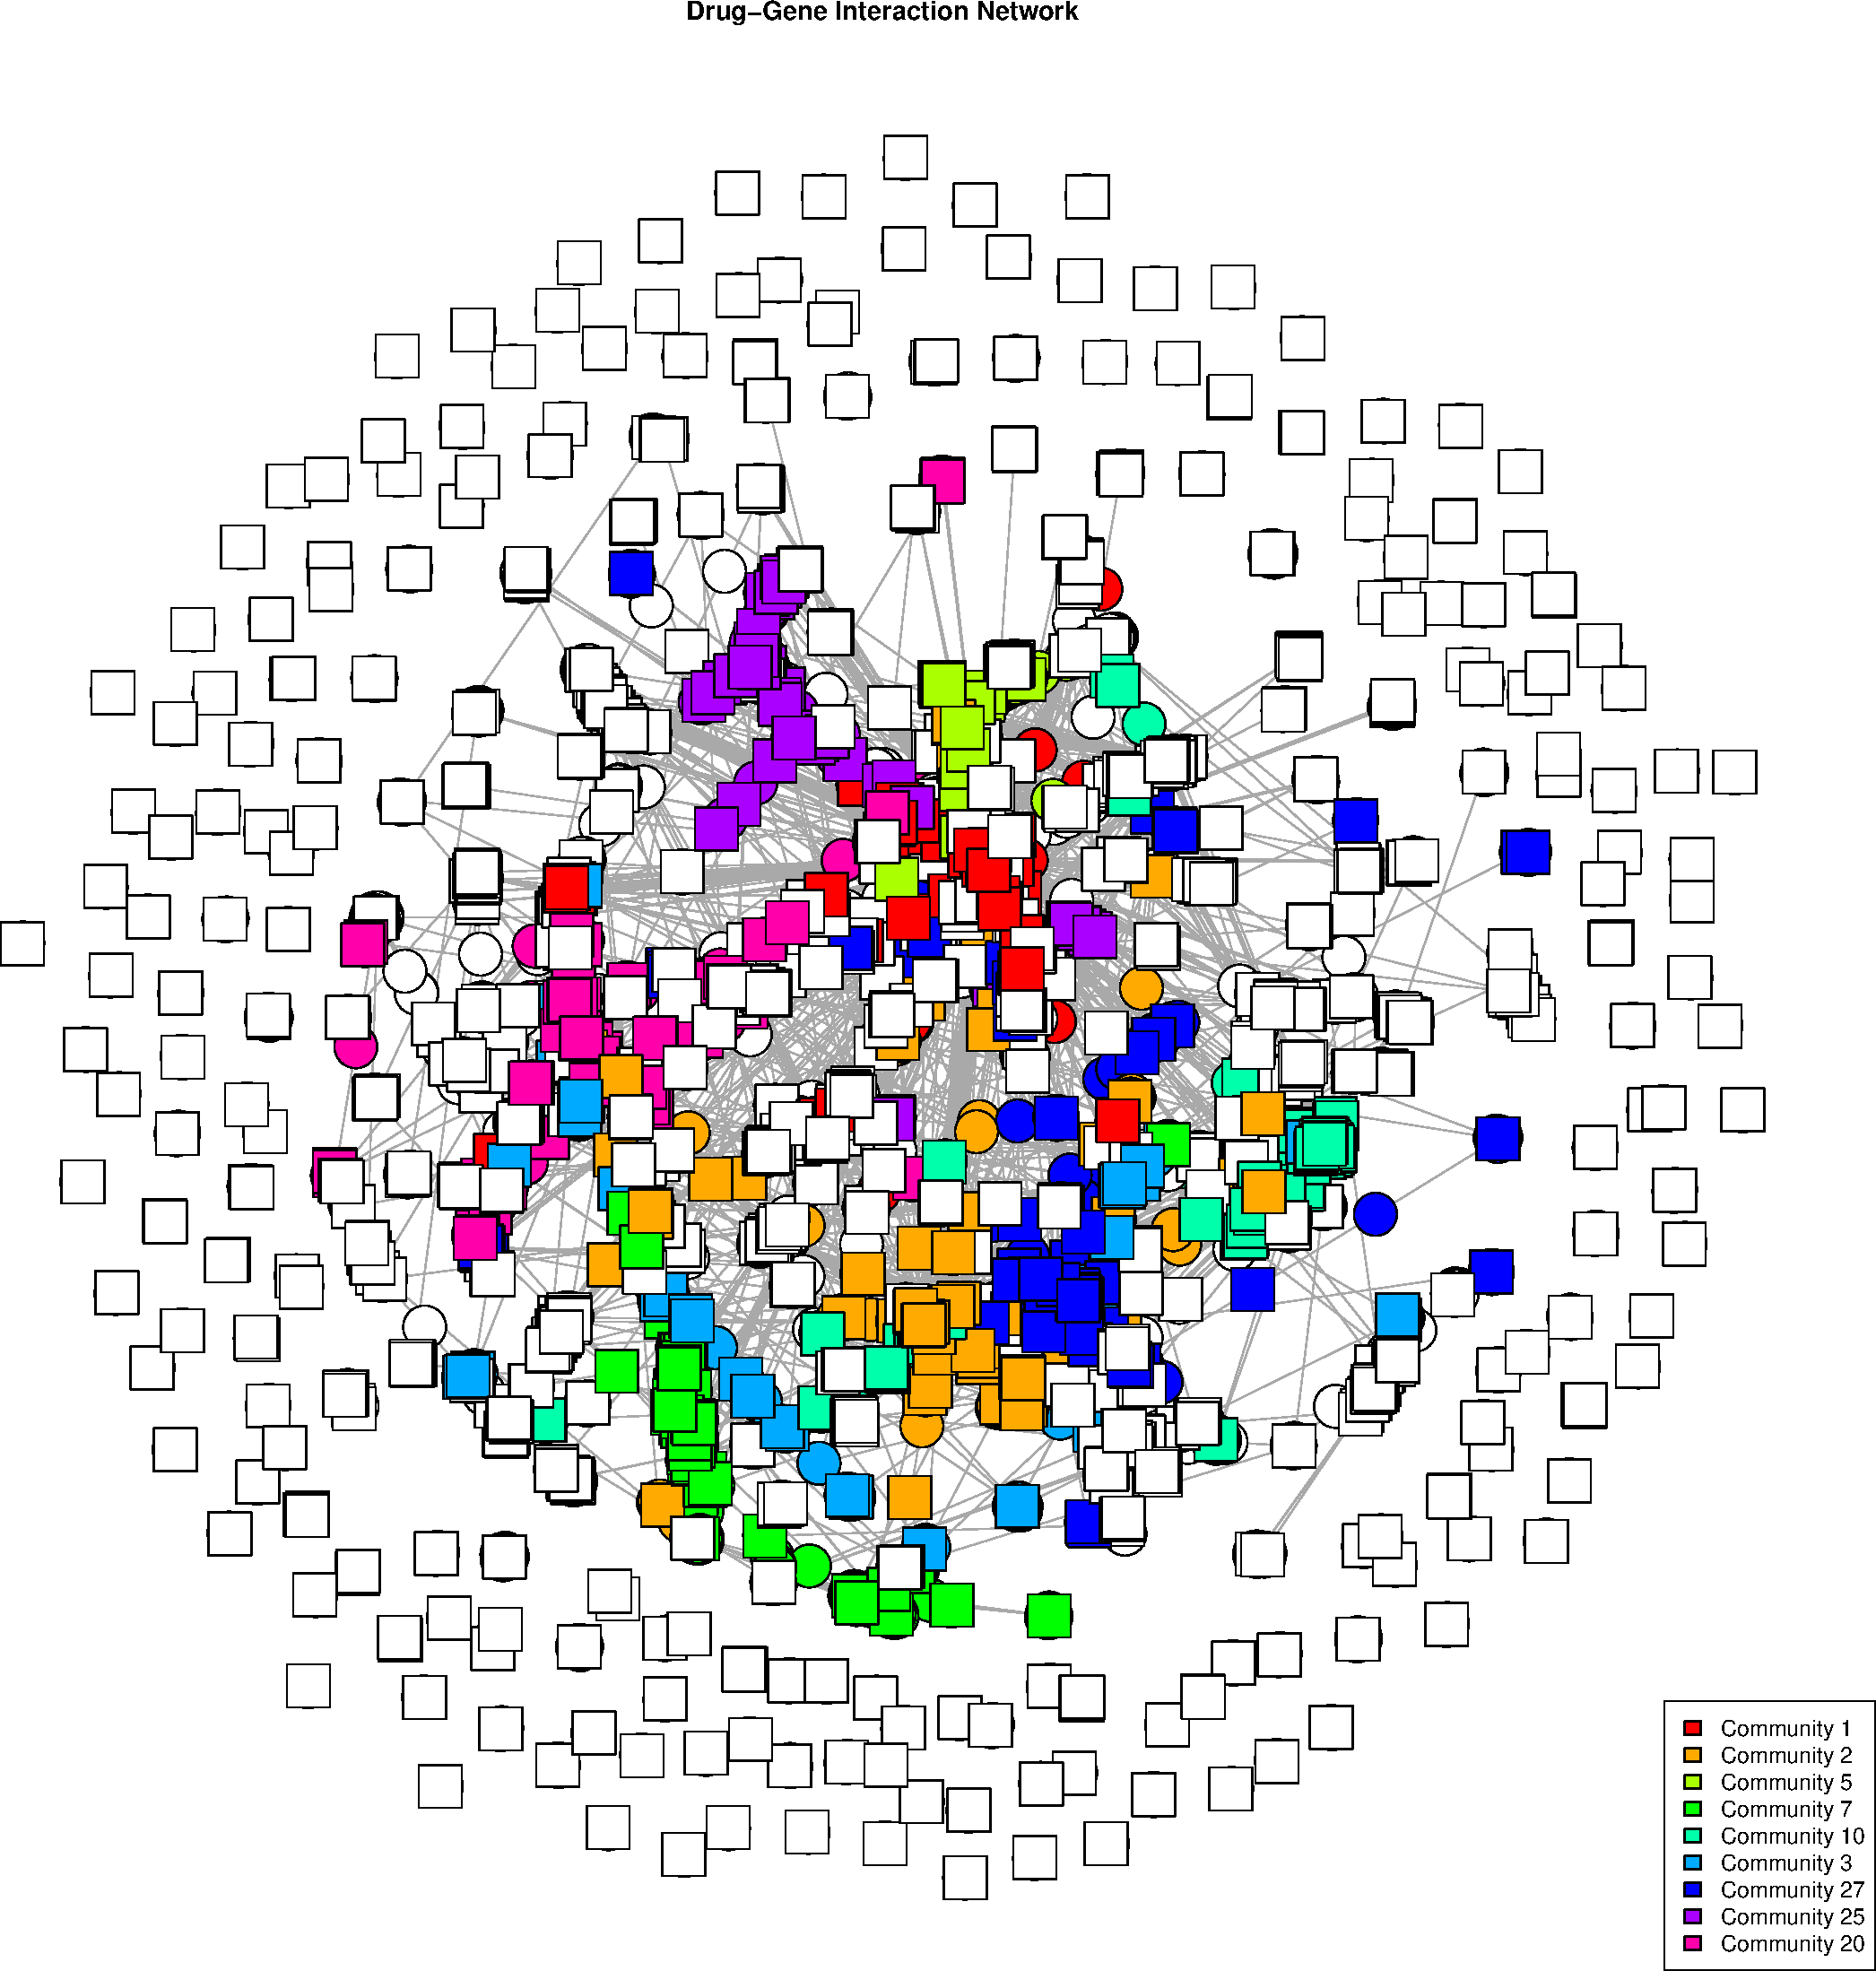
\includegraphics{lab5bio_files/figure-latex/plot1-1.pdf}

\begin{verbatim}
## IGRAPH 2398937 UN-B 7341 15138 -- 
## + attr: name (v/c), type (v/l), shape (v/c)
## + edges from 2398937 (vertex names):
##  [1] DB00357--P05108 DB02721--P00325 DB00773--P23219 DB07138--Q16539
##  [5] DB08136--P24941 DB01242--P23975 DB01238--P08173 DB00186--P48169
##  [9] DB00338--P10635 DB01151--P08913 DB01244--P05023 DB01745--P07477
## [13] DB01996--P08254 DB04800--P18031 DB08352--Q16539 DB00133--P21549
## [17] DB00163--P21266 DB00197--P10632 DB06777--P08684 DB01151--P10635
## [21] DB00356--P08684 DB01589--P34903 DB01272--P20645 DB08846--Q14534
## [25] DB01151--P33261 DB01076--P04035 DB00605--Q03181 DB08515--P49721
## [29] DB02401--P07195 DB01057--P06276 DB03286--P11217 DB08814--Q9Y233
## + ... omitted several edges
\end{verbatim}

\subsection{Graph 2}\label{graph-2}

\begin{Shaded}
\begin{Highlighting}[]
\CommentTok{\# Function to create and plot a bipartite network from an edge matrix}
\NormalTok{plot\_bipartite\_network\_2 }\OtherTok{\textless{}{-}} \ControlFlowTok{function}\NormalTok{(edge\_matrix, }\AttributeTok{title =} \StringTok{"Bipartite Network"}\NormalTok{, }\AttributeTok{top\_n =} \DecValTok{9}\NormalTok{) \{}
  \CommentTok{\# Create unique node names}
\NormalTok{  drugs }\OtherTok{\textless{}{-}} \FunctionTok{unique}\NormalTok{(edge\_matrix[,}\DecValTok{1}\NormalTok{])}
\NormalTok{  genes }\OtherTok{\textless{}{-}} \FunctionTok{unique}\NormalTok{(edge\_matrix[,}\DecValTok{2}\NormalTok{])}
  
  \CommentTok{\# Create the graph}
\NormalTok{  g }\OtherTok{\textless{}{-}} \FunctionTok{make\_empty\_graph}\NormalTok{(}\AttributeTok{directed =} \ConstantTok{FALSE}\NormalTok{)}
  
  \CommentTok{\# Add all nodes}
\NormalTok{  all\_nodes }\OtherTok{\textless{}{-}} \FunctionTok{c}\NormalTok{(drugs, genes)}
\NormalTok{  g }\OtherTok{\textless{}{-}} \FunctionTok{add\_vertices}\NormalTok{(g, }\FunctionTok{length}\NormalTok{(all\_nodes), }\AttributeTok{name =}\NormalTok{ all\_nodes)}
  
  \CommentTok{\# Create type attribute for bipartite graph}
  \FunctionTok{V}\NormalTok{(g)}\SpecialCharTok{$}\NormalTok{type }\OtherTok{\textless{}{-}} \FunctionTok{c}\NormalTok{(}\FunctionTok{rep}\NormalTok{(}\ConstantTok{TRUE}\NormalTok{, }\FunctionTok{length}\NormalTok{(drugs)), }\FunctionTok{rep}\NormalTok{(}\ConstantTok{FALSE}\NormalTok{, }\FunctionTok{length}\NormalTok{(genes)))}
  
  \CommentTok{\# Add edges}
\NormalTok{  edges }\OtherTok{\textless{}{-}} \FunctionTok{apply}\NormalTok{(edge\_matrix, }\DecValTok{1}\NormalTok{, }\ControlFlowTok{function}\NormalTok{(x) }\FunctionTok{c}\NormalTok{(}\FunctionTok{which}\NormalTok{(}\FunctionTok{V}\NormalTok{(g)}\SpecialCharTok{$}\NormalTok{name }\SpecialCharTok{==}\NormalTok{ x[}\DecValTok{1}\NormalTok{]), }\FunctionTok{which}\NormalTok{(}\FunctionTok{V}\NormalTok{(g)}\SpecialCharTok{$}\NormalTok{name }\SpecialCharTok{==}\NormalTok{ x[}\DecValTok{2}\NormalTok{])))}
  
  \CommentTok{\# Add all edges at once}
\NormalTok{  g }\OtherTok{\textless{}{-}} \FunctionTok{add\_edges}\NormalTok{(g, }\FunctionTok{unlist}\NormalTok{(edges))}
  \CommentTok{\# Set node colors based on type}
  \CommentTok{\#V(g)$color \textless{}{-} ifelse(V(g)$type, "lightblue", "lightgreen")}
  
\NormalTok{  comms }\OtherTok{\textless{}{-}} \FunctionTok{cluster\_louvain}\NormalTok{(g)}
\NormalTok{  freq\_memb }\OtherTok{\textless{}{-}} \FunctionTok{table}\NormalTok{(}\FunctionTok{membership}\NormalTok{(comms))}
\NormalTok{  big\_mems }\OtherTok{\textless{}{-}}\NormalTok{ freq\_memb[}\FunctionTok{order}\NormalTok{(freq\_memb,}\AttributeTok{decreasing =}\NormalTok{ T)][}\DecValTok{1}\SpecialCharTok{:}\NormalTok{top\_n]}

\NormalTok{  right\_index }\OtherTok{\textless{}{-}} \FunctionTok{as.vector}\NormalTok{(}\FunctionTok{as.numeric}\NormalTok{(}\FunctionTok{names}\NormalTok{(big\_mems)))}
\NormalTok{  mems }\OtherTok{\textless{}{-}} \FunctionTok{membership}\NormalTok{(comms)}
\NormalTok{  comm\_col }\OtherTok{\textless{}{-}} \FunctionTok{rainbow}\NormalTok{(top\_n)[mems]}
\NormalTok{  comm\_col }\OtherTok{\textless{}{-}} \FunctionTok{rep}\NormalTok{(}\StringTok{"\#FFFFFF"}\NormalTok{,}\FunctionTok{length}\NormalTok{(comm\_col))}

\NormalTok{  topncol }\OtherTok{\textless{}{-}} \FunctionTok{c}\NormalTok{(}\StringTok{"\#FF0000"}\NormalTok{, }\StringTok{"\#FFAA00"}\NormalTok{, }\StringTok{"\#AAFF00"}\NormalTok{, }\StringTok{"\#00FF00"}\NormalTok{ ,}\StringTok{"\#00FFAA"}\NormalTok{,}
               \StringTok{"\#00AAFF"}\NormalTok{, }\StringTok{"\#0000FF"}\NormalTok{ ,}\StringTok{"\#AA00FF"}\NormalTok{, }\StringTok{"\#FF00AA"}\NormalTok{)}

  \ControlFlowTok{for}\NormalTok{(i }\ControlFlowTok{in} \DecValTok{1}\SpecialCharTok{:}\FunctionTok{length}\NormalTok{(right\_index)) \{}
\NormalTok{    comm\_col[}\FunctionTok{which}\NormalTok{(mems }\SpecialCharTok{==}\NormalTok{ right\_index[i])] }\OtherTok{\textless{}{-}}\NormalTok{ topncol[i]}
\NormalTok{  \}}
  

  \CommentTok{\# Plot the network}
  
  \FunctionTok{plot}\NormalTok{(g, }
       \AttributeTok{vertex.label =} \FunctionTok{V}\NormalTok{(g)}\SpecialCharTok{$}\NormalTok{name,}
       \AttributeTok{vertex.color =}\NormalTok{ comm\_col,}
       \AttributeTok{vertex.label.cex =} \FloatTok{0.1}\NormalTok{,  }\CommentTok{\# Adjust label size}
       \AttributeTok{vertex.size =} \DecValTok{5}\NormalTok{,         }\CommentTok{\# Node size}
       \AttributeTok{vertex.label.color =} \StringTok{"black"}\NormalTok{,}
       \AttributeTok{main =}\NormalTok{ title,}
       \AttributeTok{layout =}\NormalTok{ layout\_as\_bipartite  }\CommentTok{\# Specific layout for bipartite graphs}
\NormalTok{  )}
  \FunctionTok{legend}\NormalTok{(}\StringTok{"bottomright"}\NormalTok{, }\AttributeTok{legend =} \FunctionTok{paste}\NormalTok{(}\StringTok{"Community"}\NormalTok{, right\_index),}
           \AttributeTok{fill =}\NormalTok{ topncol)}
  \CommentTok{\# Return the graph object for further analysis if needed}
  \FunctionTok{return}\NormalTok{(g)}
\NormalTok{\}}

\CommentTok{\# Example usage:}
\CommentTok{\# Create a sample edge matrix (drug{-}gene connections)}
\NormalTok{edge\_matrix }\OtherTok{\textless{}{-}}\NormalTok{ data}

\CommentTok{\# Plot the network}
\FunctionTok{plot\_bipartite\_network\_2}\NormalTok{(edge\_matrix, }\StringTok{"Drug{-}Gene Interaction Network"}\NormalTok{)}
\end{Highlighting}
\end{Shaded}

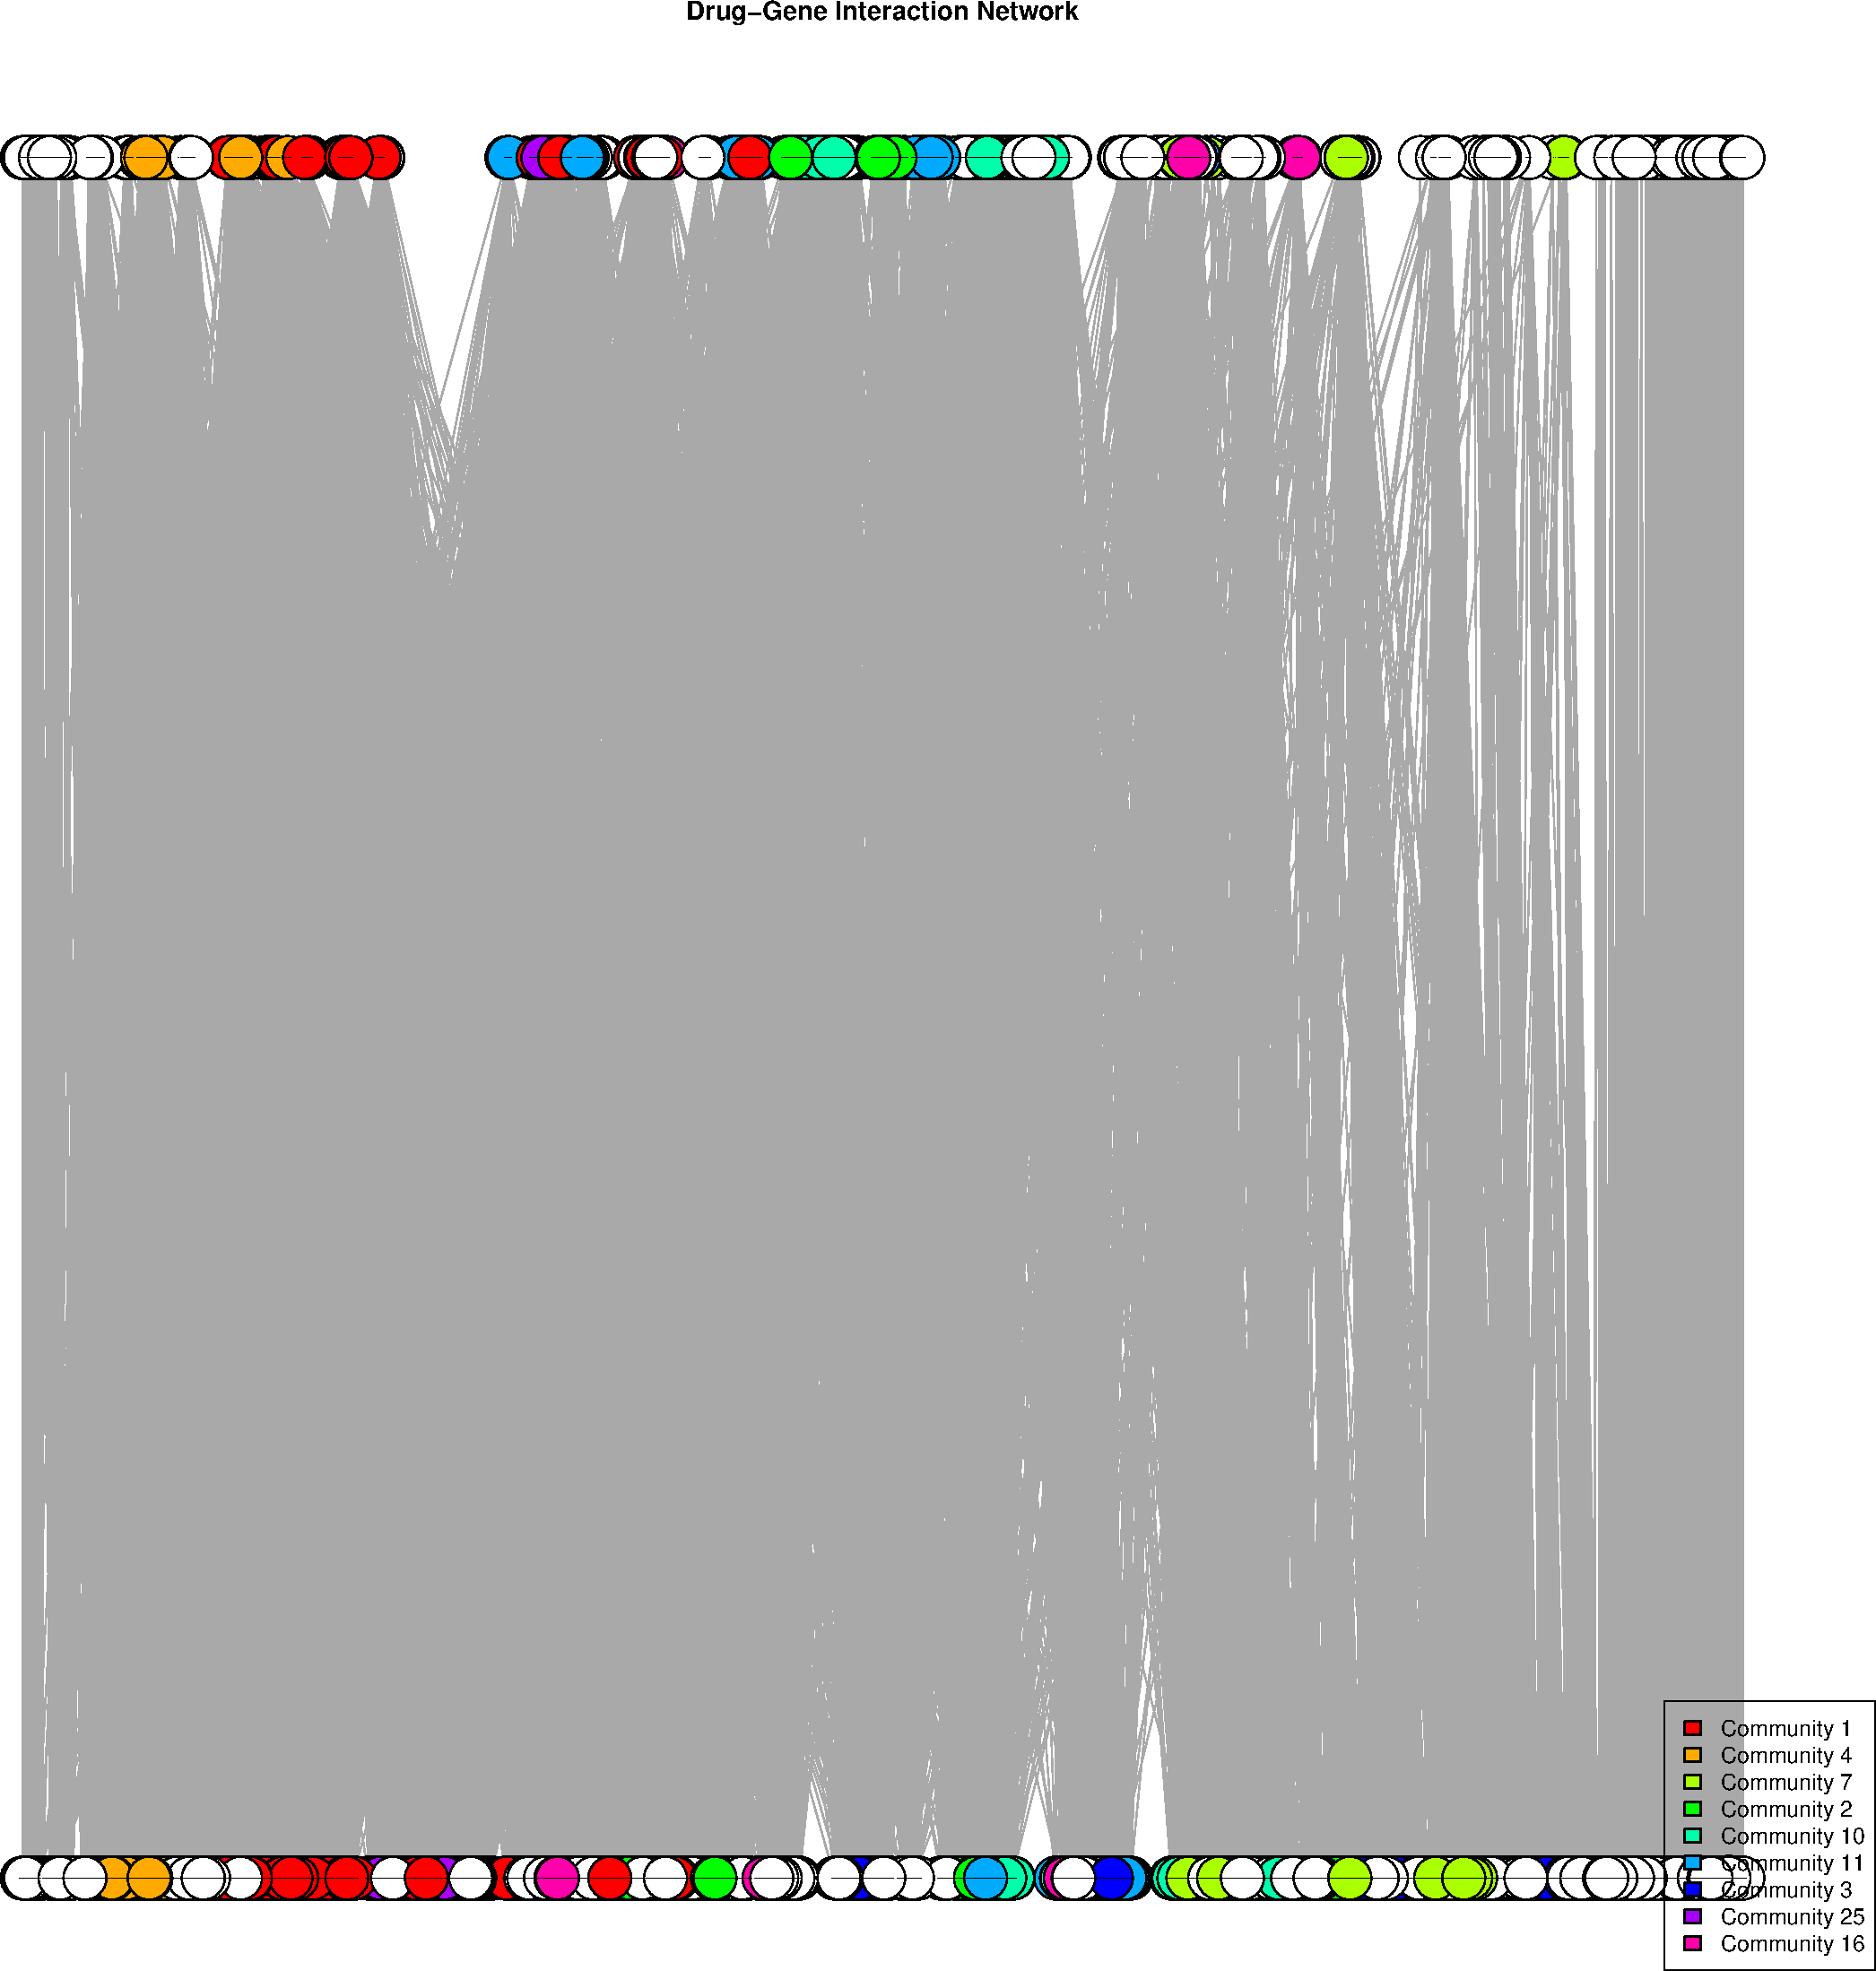
\includegraphics{lab5bio_files/figure-latex/plot2-1.pdf}

\begin{verbatim}
## IGRAPH 2e4ce70 UN-B 7341 15138 -- 
## + attr: name (v/c), type (v/l)
## + edges from 2e4ce70 (vertex names):
##  [1] DB00357--P05108 DB02721--P00325 DB00773--P23219 DB07138--Q16539
##  [5] DB08136--P24941 DB01242--P23975 DB01238--P08173 DB00186--P48169
##  [9] DB00338--P10635 DB01151--P08913 DB01244--P05023 DB01745--P07477
## [13] DB01996--P08254 DB04800--P18031 DB08352--Q16539 DB00133--P21549
## [17] DB00163--P21266 DB00197--P10632 DB06777--P08684 DB01151--P10635
## [21] DB00356--P08684 DB01589--P34903 DB01272--P20645 DB08846--Q14534
## [25] DB01151--P33261 DB01076--P04035 DB00605--Q03181 DB08515--P49721
## [29] DB02401--P07195 DB01057--P06276 DB03286--P11217 DB08814--Q9Y233
## + ... omitted several edges
\end{verbatim}

\begin{Shaded}
\begin{Highlighting}[]
\NormalTok{top\_n }\OtherTok{\textless{}{-}} \DecValTok{9}
\NormalTok{communitys }\OtherTok{\textless{}{-}} \FunctionTok{plot\_bipartite\_network}\NormalTok{(edge\_matrix, }\AttributeTok{plot\_graph =} \ConstantTok{FALSE}\NormalTok{)}
\NormalTok{freq\_memb }\OtherTok{\textless{}{-}} \FunctionTok{table}\NormalTok{(}\FunctionTok{membership}\NormalTok{(communitys))}
\NormalTok{big\_mems }\OtherTok{\textless{}{-}}\NormalTok{ freq\_memb[}\FunctionTok{order}\NormalTok{(freq\_memb,}\AttributeTok{decreasing =}\NormalTok{ T)][}\DecValTok{1}\SpecialCharTok{:}\NormalTok{top\_n]}

\NormalTok{right\_index }\OtherTok{\textless{}{-}} \FunctionTok{as.vector}\NormalTok{(}\FunctionTok{as.numeric}\NormalTok{(}\FunctionTok{names}\NormalTok{(big\_mems)))}



\NormalTok{biggest\_com }\OtherTok{\textless{}{-}}\NormalTok{ communitys[[right\_index[}\DecValTok{1}\NormalTok{]]]}


\CommentTok{\# install.packages("BiocManager")}
\CommentTok{\# BiocManager::install("clusterProfiler")}
\CommentTok{\# BiocManager::install("org.Hs.eg.db")}
\CommentTok{\# devtools::install\_github("YuLab{-}SMU/clusterProfiler")}

\FunctionTok{library}\NormalTok{(clusterProfiler)}
\end{Highlighting}
\end{Shaded}

\begin{verbatim}
## 
\end{verbatim}

\begin{verbatim}
## clusterProfiler v4.15.1.001 Learn more at https://yulab-smu.top/contribution-knowledge-mining/
## 
## Please cite:
## 
## S Xu, E Hu, Y Cai, Z Xie, X Luo, L Zhan, W Tang, Q Wang, B Liu, R Wang,
## W Xie, T Wu, L Xie, G Yu. Using clusterProfiler to characterize
## multiomics data. Nature Protocols. 2024, doi:10.1038/s41596-024-01020-z
\end{verbatim}

\begin{verbatim}
## 
## Attaching package: 'clusterProfiler'
\end{verbatim}

\begin{verbatim}
## The following object is masked from 'package:igraph':
## 
##     simplify
\end{verbatim}

\begin{verbatim}
## The following object is masked from 'package:stats':
## 
##     filter
\end{verbatim}

\begin{Shaded}
\begin{Highlighting}[]
\FunctionTok{library}\NormalTok{(org.Hs.eg.db)}
\end{Highlighting}
\end{Shaded}

\begin{verbatim}
## Loading required package: AnnotationDbi
\end{verbatim}

\begin{verbatim}
## Loading required package: stats4
\end{verbatim}

\begin{verbatim}
## Loading required package: BiocGenerics
\end{verbatim}

\begin{verbatim}
## 
## Attaching package: 'BiocGenerics'
\end{verbatim}

\begin{verbatim}
## The following objects are masked from 'package:igraph':
## 
##     normalize, path, union
\end{verbatim}

\begin{verbatim}
## The following objects are masked from 'package:stats':
## 
##     IQR, mad, sd, var, xtabs
\end{verbatim}

\begin{verbatim}
## The following objects are masked from 'package:base':
## 
##     anyDuplicated, aperm, append, as.data.frame, basename, cbind,
##     colnames, dirname, do.call, duplicated, eval, evalq, Filter, Find,
##     get, grep, grepl, intersect, is.unsorted, lapply, Map, mapply,
##     match, mget, order, paste, pmax, pmax.int, pmin, pmin.int,
##     Position, rank, rbind, Reduce, rownames, sapply, saveRDS, setdiff,
##     table, tapply, union, unique, unsplit, which.max, which.min
\end{verbatim}

\begin{verbatim}
## Loading required package: Biobase
\end{verbatim}

\begin{verbatim}
## Welcome to Bioconductor
## 
##     Vignettes contain introductory material; view with
##     'browseVignettes()'. To cite Bioconductor, see
##     'citation("Biobase")', and for packages 'citation("pkgname")'.
\end{verbatim}

\begin{verbatim}
## Loading required package: IRanges
\end{verbatim}

\begin{verbatim}
## Loading required package: S4Vectors
\end{verbatim}

\begin{verbatim}
## 
## Attaching package: 'S4Vectors'
\end{verbatim}

\begin{verbatim}
## The following object is masked from 'package:clusterProfiler':
## 
##     rename
\end{verbatim}

\begin{verbatim}
## The following object is masked from 'package:utils':
## 
##     findMatches
\end{verbatim}

\begin{verbatim}
## The following objects are masked from 'package:base':
## 
##     expand.grid, I, unname
\end{verbatim}

\begin{verbatim}
## 
## Attaching package: 'IRanges'
\end{verbatim}

\begin{verbatim}
## The following object is masked from 'package:clusterProfiler':
## 
##     slice
\end{verbatim}

\begin{verbatim}
## The following object is masked from 'package:grDevices':
## 
##     windows
\end{verbatim}

\begin{verbatim}
## 
## Attaching package: 'AnnotationDbi'
\end{verbatim}

\begin{verbatim}
## The following object is masked from 'package:clusterProfiler':
## 
##     select
\end{verbatim}

\begin{verbatim}
## 
\end{verbatim}

\begin{Shaded}
\begin{Highlighting}[]
\CommentTok{\# Perform GO enrichment analysis for the current community}
\NormalTok{go\_results }\OtherTok{\textless{}{-}} \FunctionTok{enrichGO}\NormalTok{(}\AttributeTok{gene =}\NormalTok{ biggest\_com,}
                       \AttributeTok{OrgDb =}\NormalTok{ org.Hs.eg.db, }\AttributeTok{keyType =} \StringTok{"UNIPROT"}\NormalTok{, }\AttributeTok{ont =} \StringTok{"BP"}\NormalTok{)}

\NormalTok{top\_go\_terms }\OtherTok{\textless{}{-}}\NormalTok{ go\_results}\SpecialCharTok{@}\NormalTok{result[}\FunctionTok{order}\NormalTok{(go\_results}\SpecialCharTok{@}\NormalTok{result}\SpecialCharTok{$}\NormalTok{p.adjust), ]}
\FunctionTok{head}\NormalTok{(top\_go\_terms}\SpecialCharTok{$}\NormalTok{Description, }\DecValTok{10}\NormalTok{) }\CommentTok{\# strongly related to neurobiology}
\end{Highlighting}
\end{Shaded}

\begin{verbatim}
##  [1] "estrogen metabolic process"            
##  [2] "epoxygenase P450 pathway"              
##  [3] "arachidonate metabolic process"        
##  [4] "cellular glucuronidation"              
##  [5] "uronic acid metabolic process"         
##  [6] "glucuronate metabolic process"         
##  [7] "xenobiotic catabolic process"          
##  [8] "toxin metabolic process"               
##  [9] "retinoic acid metabolic process"       
## [10] "regulation of cellular glucuronidation"
\end{verbatim}

\begin{Shaded}
\begin{Highlighting}[]
\FunctionTok{barplot}\NormalTok{(go\_results, }\AttributeTok{showCategory =} \DecValTok{10}\NormalTok{)}
\end{Highlighting}
\end{Shaded}

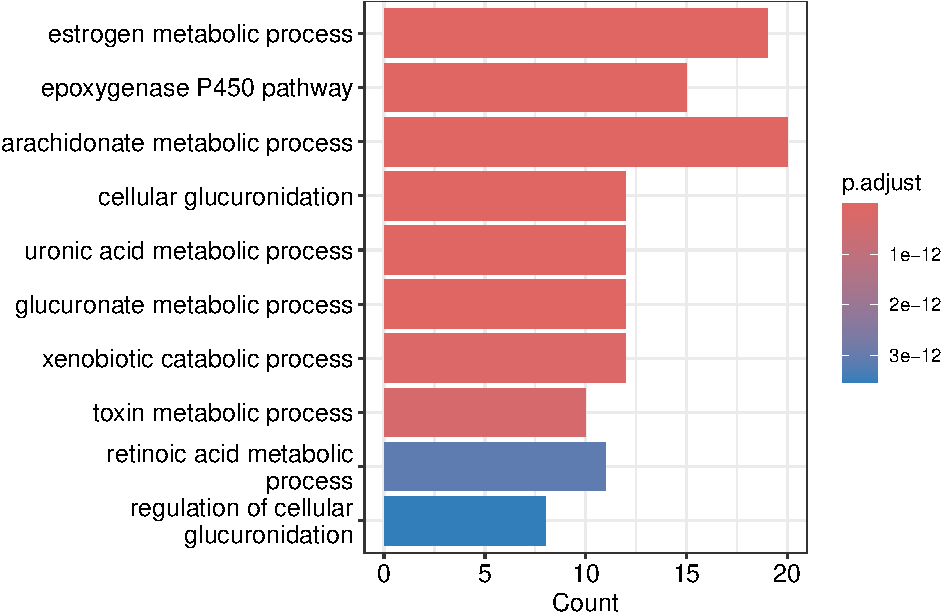
\includegraphics{lab5bio_files/figure-latex/first_com-1.pdf}

\begin{Shaded}
\begin{Highlighting}[]
\NormalTok{sec\_biggest\_com }\OtherTok{\textless{}{-}}\NormalTok{ communitys[[right\_index[}\DecValTok{2}\NormalTok{]]]}


\CommentTok{\# Perform GO enrichment analysis for the current community}
\NormalTok{go\_results }\OtherTok{\textless{}{-}} \FunctionTok{enrichGO}\NormalTok{(}\AttributeTok{gene =}\NormalTok{ sec\_biggest\_com,}
                       \AttributeTok{OrgDb =}\NormalTok{ org.Hs.eg.db, }\AttributeTok{keyType =} \StringTok{"UNIPROT"}\NormalTok{, }\AttributeTok{ont =} \StringTok{"BP"}\NormalTok{)}

\NormalTok{top\_go\_terms }\OtherTok{\textless{}{-}}\NormalTok{ go\_results}\SpecialCharTok{@}\NormalTok{result[}\FunctionTok{order}\NormalTok{(go\_results}\SpecialCharTok{@}\NormalTok{result}\SpecialCharTok{$}\NormalTok{p.adjust), ]}
\FunctionTok{head}\NormalTok{(top\_go\_terms}\SpecialCharTok{$}\NormalTok{Description, }\DecValTok{10}\NormalTok{) }
\end{Highlighting}
\end{Shaded}

\begin{verbatim}
##  [1] "G protein-coupled serotonin receptor signaling pathway"                                     
##  [2] "G protein-coupled receptor signaling pathway, coupled to cyclic nucleotide second messenger"
##  [3] "adenylate cyclase-activating adrenergic receptor signaling pathway"                         
##  [4] "catecholamine transport"                                                                    
##  [5] "adrenergic receptor signaling pathway"                                                      
##  [6] "dopamine transport"                                                                         
##  [7] "cellular response to dopamine"                                                              
##  [8] "response to dopamine"                                                                       
##  [9] "adenylate cyclase-inhibiting serotonin receptor signaling pathway"                          
## [10] "cellular response to monoamine stimulus"
\end{verbatim}

\begin{Shaded}
\begin{Highlighting}[]
\FunctionTok{barplot}\NormalTok{(go\_results, }\AttributeTok{showCategory =} \DecValTok{10}\NormalTok{)}
\end{Highlighting}
\end{Shaded}

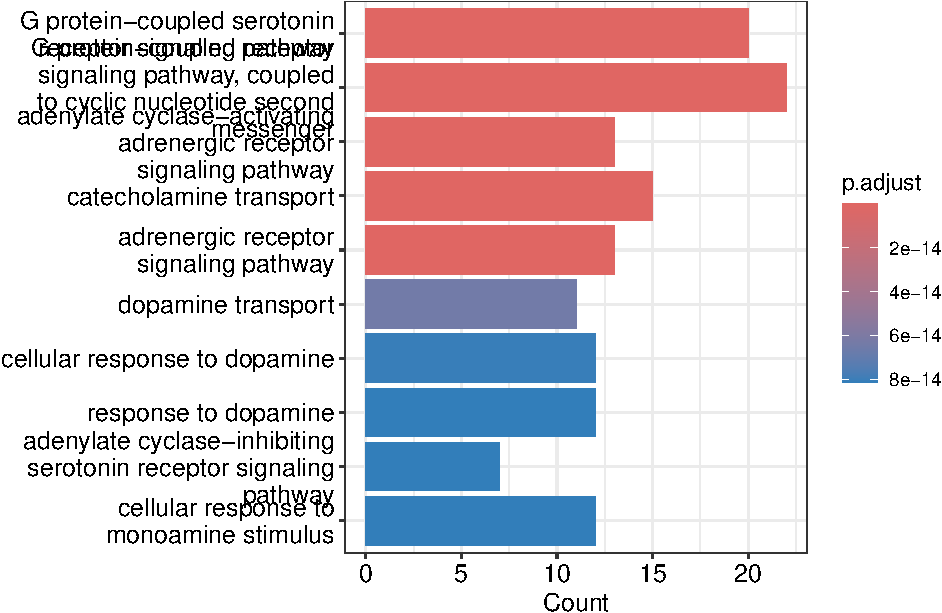
\includegraphics{lab5bio_files/figure-latex/sec_com-1.pdf}

\section{Question 2}\label{question-2}

Recreate one of the three analyses that can be found on
\url{https://strimmerlab.github.io/software/genenet/index.html}.
Document and discuss all your steps. In the analyses there is the step
where you select the edges to keep. There a particular criterion is
chosen for edge inclusion. Vary this criterion and explore how the
resulting clusters will differ with the changes. Take one found cluster,
identify the elements in it and try to find information on this cluster.
Is it related to some known biological phenomena? If you do not find
anything, then document your search attempts.

\end{document}
